%%%%
% Преамбула: подключение необходимых пакетов
% Редактируйте осторожно!
%

\documentclass[hyperref={unicode}]{beamer}

\usepackage{listings}  
\usepackage[utf8x]{inputenc}
\usepackage[english, russian]{babel}
\usepackage{color, colortbl}
\usepackage{rotating} 
\usepackage{graphicx}
\usepackage{algorithmic}

\usetheme[nosecheader]{PetrSU-CS}


%%%%
% Преамбула: основные параметры презентации
% Отредактируйте в соответствии с комментариями
%

\title[%
    % Краткое название работы не используется в этой презентации!
    Бобры и Интернет
]{%
    % Полное название работы отображается на титульной странице
	Реализация мобильного приложения \\
	интеллектуального персонифицированного\\
	геолокационного трекера пользователя
}

% Подзаголовком опишите тип работы:
% - Курсовая работа
% - Выпускная квалификационная работа бакалавра
% - Дипломная работа
% - Магистерская диссертация
\subtitle{Отчет о научно-исследовательской работе}

\author[%
    % Имя и фамилия автора работы отображаются на каждом слайде в нижнем колонтитуле
    Владислав Клименко
]{%
    % Имя, отчество и фамилия автора работы отображаются на титульном слайде
    Владислав Викторович Клименко
}

\date[%
    % Дата защиты
    01.06.2018
]{%
    % Руководитель
    Научный руководитель: преподаватель  В. М. Димитров
}

\institute[%
    % Краткое название организации не используется в этой презентации
    ПетрГУ
]{%
    % Полное название организации и подразделения
    Петрозаводский государственный университет\\
    Кафедра информатики и математического обеспечения
}


%%%%
%
% Начало содержимого слайдов
%

\begin{document}

% Титульный слайд
\begin{frame}
\maketitle
\end{frame}

% Пример слайда для обоснования актуальности работы
\begin{frame}
  % Заголовок слайда
  \frametitle{Основные понятия}
  Трекер(Геотрекер) - это программа позволяющая отслеживать путь пользователя и выводить
  различную информацию о том, каким образом он перемещался.
  
  Трек - это путь, который прошёл человек не останавливаясь.
\end{frame}

% Пример слайда с формулировкой целей и задач
\begin{frame}
  % Заголовок слайда
  \frametitle{Цель и задачи}
  \begin{block}{Цель работы}
    Разработать энергоэффективный трекер, который может
    постоянно опрашивать координаты пользователя и сам определять треки
  \end{block}
  \begin{block}{Задачи}
  \begin{itemize}
  	\item Написать тестовое приложение для выбора оптимальной частоты опроса.
  	\item Разработать алгоритм определения треков.
  	\item Написать основное приложение.
  \end{itemize}
  \end{block}
\end{frame}

% Пример слайда содержащего код
\begin{frame}
% Заголовок слайда
\frametitle{Обзор рынка}
Наиболее популярные геотрекеры вынуждают пользователя вручную запускать запись трека:
\begin{itemize}
	\item A-GPS Tracker
	\item Sportractive GPS Running Cycling Distance Tracker
	\item Geo Tracker - GPS tracker
	\item GPS Sports Tracker App: running, walking, cycling
\end{itemize}

\end{frame}
% Пример слайда содержащего код
\begin{frame}
% Заголовок слайда
\frametitle{Уровень энергопотребления}
Исследования проводились при следующих условий:
\begin{itemize}
	\item Устройство - ZTE Blade X3
	\item ОС - Android 5.1
	\item Google Play Services 49
\end{itemize}

\end{frame}

\begin{frame}
  % Заголовок слайда
  \frametitle{Уровень энергопотребления}
	\begin{center}
		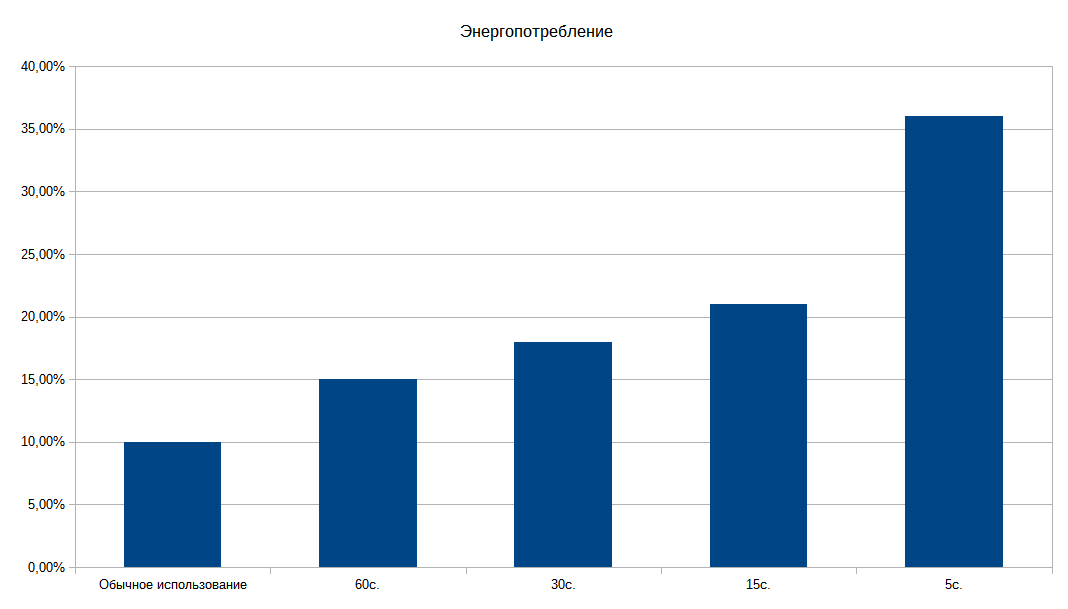
\includegraphics[width=0.8\textwidth]{images/Consuming.png}
	\end{center}
  
\end{frame}

% Пример слайда содержащего код
\begin{frame}[fragile]
% Заголовок слайда
\frametitle{Алгоритм разбиения на треки}
\framesubtitle{Код для определения точки остановки}

\begin{lstlisting}
CheckSpeed:
  dist = sqrt(111.1111111111 * ((x1 - x2) ^ 2 + 
   cos((x1 + x2) / 2) * (y1 - y2) ^ 2))
  time = to_hourse(t1 - t2)
  return dist / time <= 2 or
    dist / time >= 150
\end{lstlisting}

\end{frame}

\begin{frame}[fragile]
\frametitle{Алгоритм разбиения на треки}
\framesubtitle{Модифицированный алгоритм для определения точки остановки}

\begin{lstlisting}
checkSpeed:
  dist = 0;
  time = 0;
  for i in len(points):
    x1, y1, t1= points.get(i)
    x2, y2, t2 = points.get(i % len(points))
    dist += sqrt(111.1111111111 * ((x1 - x2) ^ 2 + 
      cos((x1 + x2) / 2) * (y1 - y2) ^ 2))
    time += to_hourse(t1 - t2)
  return dist / time < lim or
   dist / time > 120
\end{lstlisting}

\end{frame}
% Пример заключительного слайда
\begin{frame}
  \frametitle{Заключение}
  
  Полученные результаты
  
  \begin{itemize}
  	\item Найдена оптимальная частота опроса
  	\item Разработан алгоритм разбиения координат на треки
  	\item Написано основное приложение
  \end{itemize}
  
\end{frame}

% Пример слайда содержащего код
\begin{frame}
% Заголовок слайда
\frametitle{Скриншот приложения}
\begin{center}
	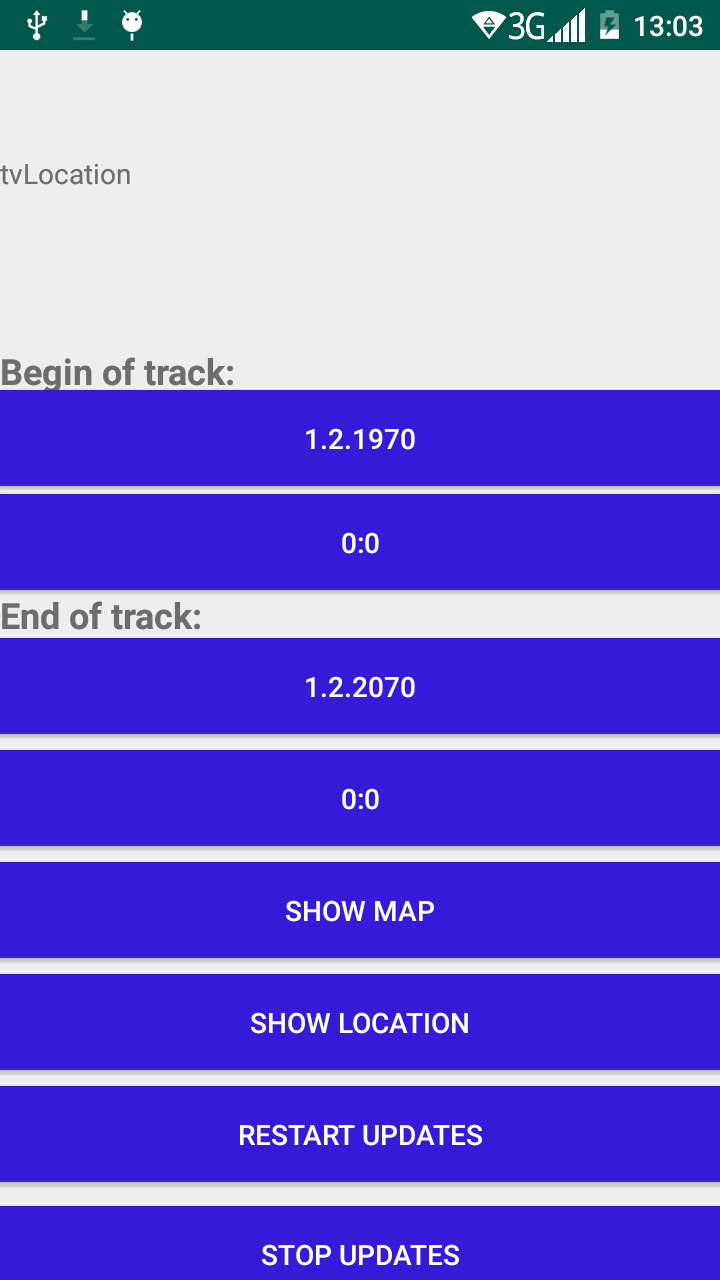
\includegraphics[height=0.8\textheight]{images/Screen_time1.png}
	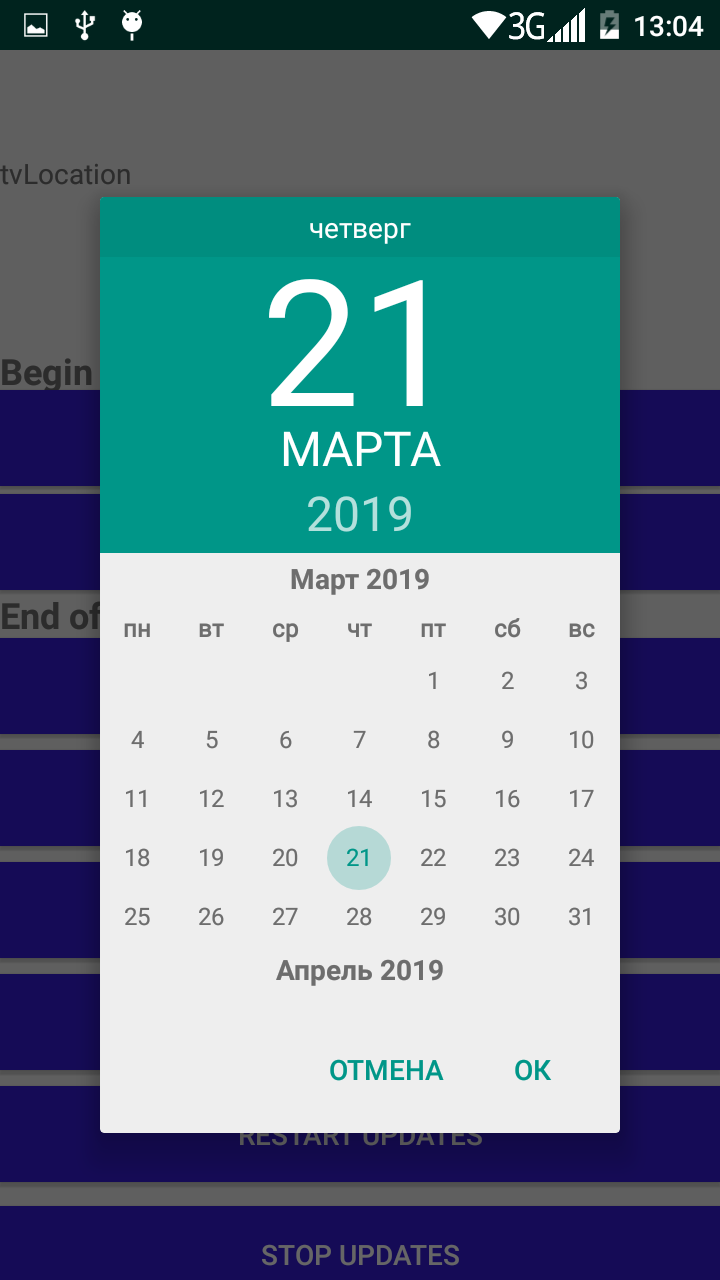
\includegraphics[height=0.8\textheight]{images/Screen_time2.png}
\end{center}

\end{frame}

% Пример слайда содержащего код
\begin{frame}
% Заголовок слайда
\frametitle{Скриншот приложения}
\begin{center}
	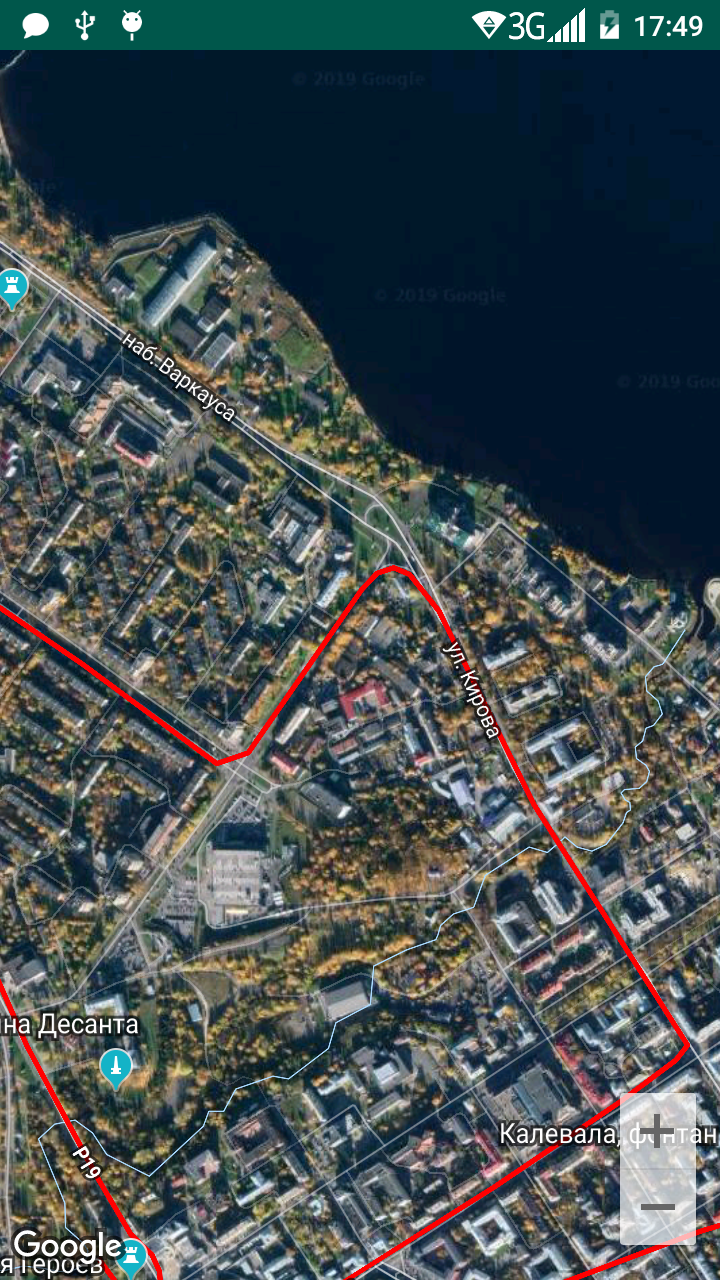
\includegraphics[height=0.8\textheight]{images/Screenshot.png}
\end{center}

\end{frame}

\begin{frame}
  \frametitle{}
  
{\Large\mbox{}\hfil Спасибо за внимание!}
  
\end{frame}
\end{document}
